\section{Auswertung}
\label{sec:Auswertung}

Im folgenden werden die Daten analysiert, die während einer Messzeit von ungefähr $T_{Messung} = 4,7  \unit\day$ aufgenommen wurden.

\subsection{Kalibrierung der Messgeräte}

Bei der Kalibrierung der Geräte trat ein Problem bei der Einstellung der Pulsdauer auf.
Aus diesem Grund wurde die Pulsdauer statt auf $10 \unit{\nano\second}$ und $20 \unit{\nano\second}$ auf $20 \unit{\nano\second}$ und $30 \unit{\nano\second}$ eingestellt.
Die Messdaten dazu sind im Anhang in \autoref{tab:20ns_table} und \autoref{tab:30ns_table} zu finden.
Die Plots der Daten und der entsprechenden Halbwertsbreiten sind in \autoref{fig:20ns_plot} und \autoref{fig:30ns_plot} abgebildet.
Auch bei der Aufnahme der Daten kam es zu Problemen, siehe dafür \autoref{sec:Diskussion}.
Hier sei allerdings angemerkt, dass die Halbwertsbreiten deshalb nur abgeschätzt werden können.
Für eine Pulsdauer von $20 \unit{\nano\second}$ ergibt sich eine Halbwertsbreite von $\Delta_\text{Breite} = 25 \unit{\nano\second}$, woraus sich dann eine Verzögerung von
\begin{equation*}
    (2 \cdot 20 - 25) \unit{\nano\second} = 15 \unit{\nano\second}  
\end{equation*}
ergibt.
Für eine Pulsdauer von $30 \unit{\nano\second}$ ergibt sich eine Halbwertsbreite von $\Delta_\text{Breite} = 37 \unit{\nano\second}$, woraus sich dann eine Verzögerung von
\begin{equation*}
    (2 \cdot 30 - 37) \unit{\nano\second} = 23 \unit{\nano\second}  
\end{equation*}
ergibt.

\begin{figure}
    \centering
    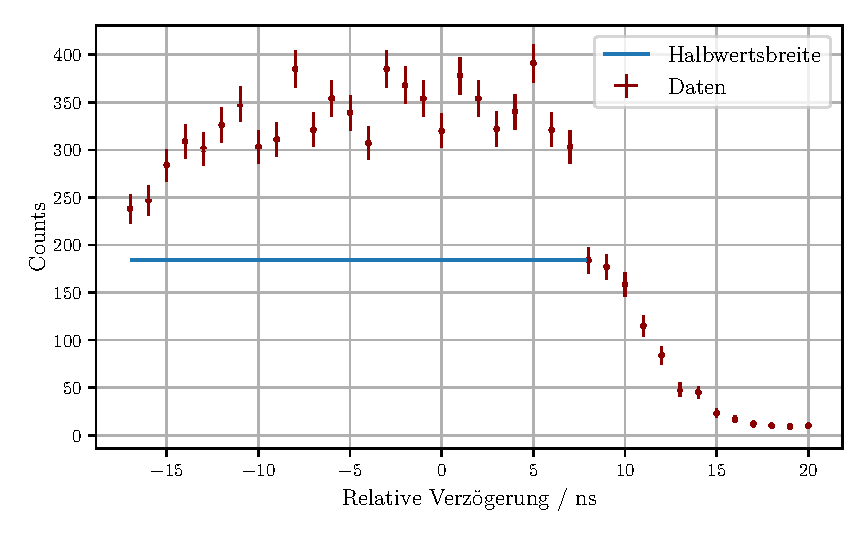
\includegraphics[width = 0.7 \linewidth]{build/20ns_plot.pdf}
    \caption{Plot zur Messung bei einer Pulsdauer von $20$ns.}
    \label{fig:20ns_plot}
\end{figure}

\begin{figure}
    \centering
    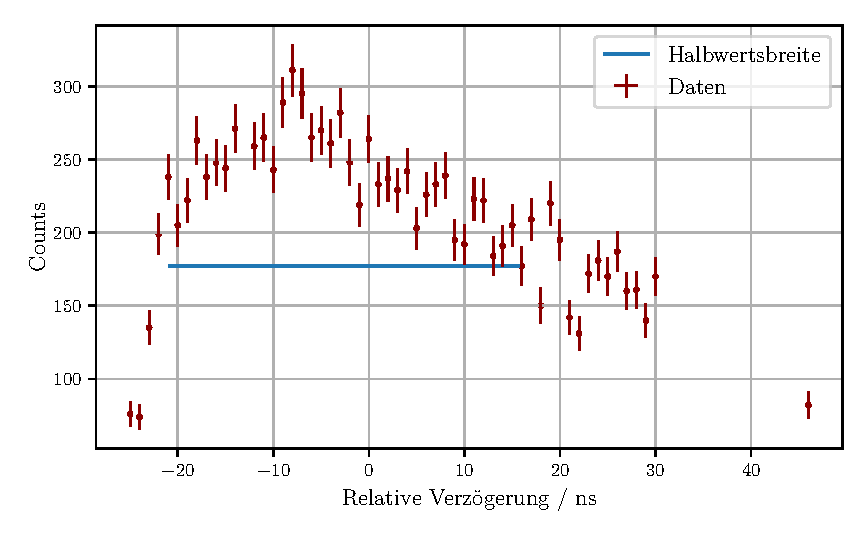
\includegraphics[width = 0.7 \linewidth]{build/30ns_plot.pdf}
    \caption{Plot zur Messung bei einer Pulsdauer von $30$ns.}
    \label{fig:30ns_plot}
\end{figure}

\subsection{Bestimmung der Zeiteinteilung der Bins am TCA} \label{sec:zeiteinteilung}

Die Messdaten sind in \autoref{tab:zeiteinteilung} zu finden.
Um den Bins des TCAs eine Zeit zuzuordnen, wird eine Regressionsrechnung durchgeführt.
Dafür wird der Ansatz
\begin{equation*}
    t = m \cdot b + c
\end{equation*}
gewählt.
Der entsprechende Plot ist in \autoref{fig:zeiteinteilung} abgebildet.
Der Fit ergibt 
$m = (0.02257 \pm 0.00005)\unit\second$ und $c = (0.148 \pm 0.006)\unit\second$.


\begin{figure}%
    \begin{subfigure}{0.68\textwidth}%
    \centering%
    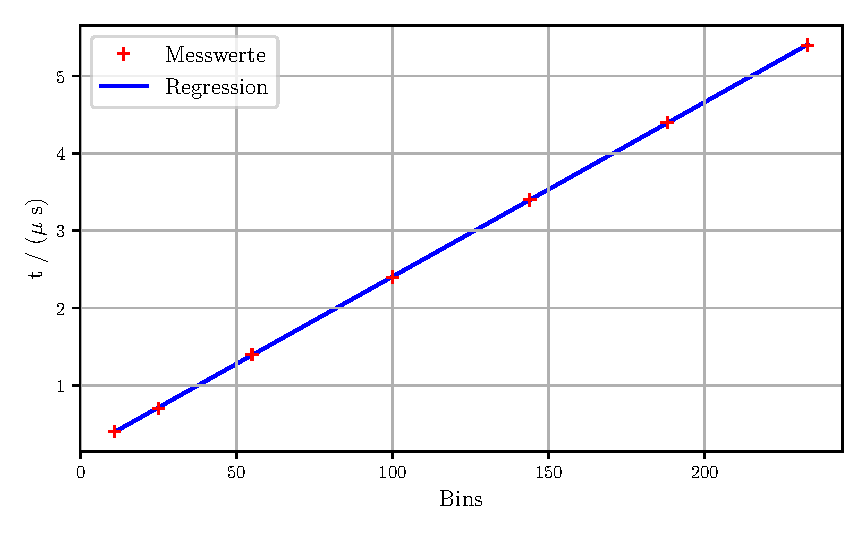
\includegraphics[width=\textwidth]{build/zeiteinteilung.pdf}%
    \caption{Fit an die Daten.}%
    \label{fig:zeiteinteilung}%
    \end{subfigure}%
    \hfill% Fills available space in the center -> space between figures
    \begin{subtable}{0.28\textwidth}%
        \centering
        \begin{tabular}{c c}
        \toprule
        Zeit &  Bins \\
        \midrule
         5,4 & 233,0 \\
         4,4 & 188,0 \\
         3,4 & 144,0 \\
         2,4 & 100,0 \\
         1,4 &  55,0 \\
         0,7 &  25,0 \\
         0,4 &  11,0 \\
        \bottomrule
        \end{tabular}
        \caption{Messdaten.}
        \label{tab:zeiteinteilung}
    \end{subtable}%
    \caption{Bestimmung der Zeiteinteilung der Bins.}
    \label{subfig:zeiteinteilung}    
\end{figure}%
    
\subsection{Bestimmung der Lebenszeit von Myonen}

\begin{figure}%
    \begin{subfigure}{0.48\textwidth}%
    \centering%
    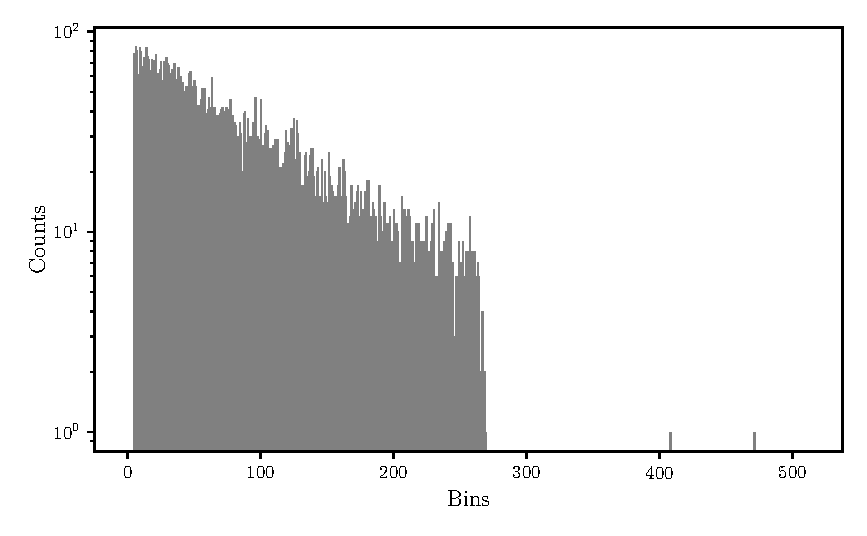
\includegraphics[width=\textwidth]{build/myonenhist.pdf}%
    \caption{Histogramm der Messdaten.}%
    \label{fig:histogramm}%
    \end{subfigure}%
    \hfill% Fills available space in the center -> space between figures
    \begin{subfigure}{0.48\textwidth}%
        \centering%
        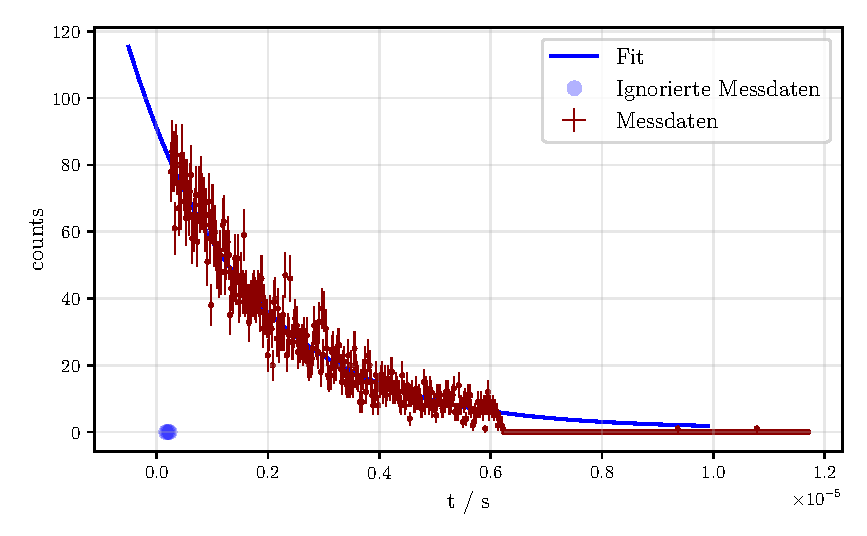
\includegraphics[width=\textwidth]{build/myonenfit.pdf}%
        \caption{Fit an die Daten.}%
        \label{fig:myonenfit}%
        \end{subfigure}%
    \caption{Abbildungen zur Ermittlung der Lebenszeit eines Myons.}
    \label{subfig:myonen}    
\end{figure}%

Die Messdaten zu diesem Versuch sind im Anhang in \autoref{tab:messdaten_myonen1}, \autoref{tab:messdaten_myonen2} und \autoref{tab:messdaten_myonen3} zu finden.
Die Daten wurden außerdem histogrammiert in \autoref{fig:histogramm} aufgetragen.
Die gezählten Ereignisse und Ereignisse, die verworfen wurden, sind in \autoref{fig:untergrund} zu sehen.
Dabei muss beachtet werden, dass der Counter einmal durchgelaufen ist.
Als Fit wird nach Vorgabe des Zerfallsgesetzes plus Untergrund die Funktion
\begin{equation*}
    N(t) = N_0 \cdot e^{- \lambda t} + U
\end{equation*} 
angesetzt.
Dabei wird stets beachtet, dass die Konstanten größer null sein müssen.
Außerdem werden die ersten vier Bins nicht beachtet, da diese mit null gefüllt sind und dies einen systematischen Fehler andeutet, siehe \autoref{sec:Diskussion}.
Der Fit ergibt $N_0 = 88.4 \pm 1.3$, $\lambda = (4.60 \pm 0.13) \cdot 10^5 \frac{1}{\unit{\second}}$ und $U = 0.0 \pm 0.4$.
Auch hier gilt dann $U \in [0 \, , \, 0,71]$, da der Untergrund nur positiv sein kann.
Der entsprechende Plot ist in \autoref{fig:myonenfit} abgebildet.
Hier wurde auch bereits mit der Formel für die Zeit aus \autoref{sec:zeiteinteilung} dem jeweiligen Bin eine Zeit zugeordnet.
Aus $\lambda$ lässt sich nun mithilfe \autoref{eq:tbd} die Lebenszeit bestimmen.
Es ergibt sich
\begin{equation}
    \tau = \frac{1}{\lambda} = (2.17 \pm 0.06) \unit{\micro\second} \, .
\end{equation}

\subsection{Bestimmung des Untergrundes} \label{sec:untergrund_ausw}

Nachdem bereits der Untergrund gefittet wurde, soll dieser auch nach der theoretischen Formel \autoref{eq:tbd} berechnet werden.
Damit ergibt sich
\begin{equation*}
    U = \frac{N_\text{Verworfen}}{N_\text{Gemessen}} = \frac{21135}{595280 + 9999999} = 0,001994 \, .
\end{equation*} 